\documentclass[11pt]{article}

\usepackage[a4paper,margin=1in]{geometry}
\usepackage{graphicx}
\usepackage{booktabs}
\usepackage{amsmath}
\usepackage{amssymb}
\usepackage{hyperref}
\usepackage{subcaption}
\usepackage{float}
\hypersetup{hidelinks}

\title{Project 1 Report: MNIST Classification with NumPy Neural Networks}
\author{Name: \textbf{Xinglei Yu} \quad Student ID: \textbf{23300290012}}
\date{May 24, 2026}

\begin{document}
\maketitle

\noindent\textbf{Code:} \href{https://github.com/spoil-ed/Neural-Network-and-Deep-Learning-PJ1}{GitHub repository}\\
\textbf{Checkpoints:} \href{https://modelscope.cn/models/imspoiled/Neural-Network-and-Deep-Learning-PJ1-Checkpoint}{ModelScope repository}

\begin{abstract}
This report studies handwritten digit classification on MNIST by implementing the main components of a neural network from scratch with NumPy. The project first builds a multi-layer perceptron (MLP) baseline, including linear-layer forward and backward propagation and softmax cross-entropy loss. It then implements a two-dimensional convolution operator and constructs a simple convolutional neural network (CNN) for comparison with the MLP. Finally, two additional directions are explored on top of both Part A and Part B models: momentum-based optimization and L2 weight decay regularization. The experiments show that the CNN baseline improves over the MLP baseline, and that momentum gives the largest performance gain for both architectures. The final CNN with momentum reaches 96.44\% test accuracy on the MNIST test set when trained on a 5000-image subset.
\end{abstract}

\section{Experimental Setup}

The purpose of this project is not only to obtain a high MNIST accuracy, but also to understand how the basic building blocks of neural networks work internally. Therefore, all model components used in the experiments are implemented directly with NumPy. No external dataset is used, and no deep-learning framework operators are called to solve the required tasks. The implemented components include a linear layer, softmax cross-entropy, a two-dimensional convolution layer, an MLP classifier, a CNN classifier, momentum optimization, and L2 weight decay.

The MNIST images are grayscale images of size $28 \times 28$, and each image belongs to one of ten digit classes. Pixel values are normalized from $[0,255]$ to $[0,1]$. To keep pure NumPy CNN training practical, I use 5000 training images and 1000 validation images sampled from the provided MNIST training set with random seed 309. Test accuracy is reported on the full 10000-image MNIST test set. This choice makes the experiments fast enough to repeat while still large enough to show meaningful differences between the models.

All experiments use batch size 64 and train for 5 epochs. The MLP and CNN baselines use stochastic gradient descent (SGD) with L2 weight decay $\lambda=10^{-4}$. The MLP baseline learning rate is 0.1, the CNN baseline learning rate is 0.05, and the momentum experiments use learning rate 0.03 with momentum coefficient $\mu=0.9$. For Part C, I apply the chosen directions to both the MLP baseline from Part A and the CNN baseline from Part B whenever the comparison is meaningful. The main comparison keeps the dataset split, epoch count, and evaluation protocol fixed so that the effect of model architecture, optimization, and regularization can be interpreted fairly.

\section{Part A: MLP Baseline}

\subsection{Required Implementation}

The MLP baseline uses the architecture
\[
784 \rightarrow 600 \rightarrow 10,
\]
with ReLU activation after the hidden linear layer. For an input batch $X \in \mathbb{R}^{N \times d}$, the linear layer computes
\[
Y = XW + b.
\]
Given upstream gradient $G=\partial L/\partial Y$, its backward pass computes
\[
\frac{\partial L}{\partial W}=X^\top G,\quad
\frac{\partial L}{\partial b}=\sum_{i=1}^{N}G_i,\quad
\frac{\partial L}{\partial X}=GW^\top.
\]

The loss function is multi-class cross-entropy with a numerically stable softmax:
\[
\mathrm{softmax}(z_i)=\frac{\exp(z_i-\max_j z_j)}{\sum_k \exp(z_k-\max_j z_j)}.
\]
For one-hot label vector $y$, the gradient with respect to logits is
\[
\frac{\partial L}{\partial z}=\frac{\mathrm{softmax}(z)-y}{N}.
\]

In the implementation, each layer stores the input from its forward pass so that the backward pass can reuse it when computing gradients. The linear layer stores its parameters in a dictionary and exposes gradients for the optimizer. This keeps the layer interface simple: the model only needs to call each layer sequentially in the forward pass and in reverse order in the backward pass. The cross-entropy layer receives logits from the model and integer class labels, converts the labels into one-hot form internally, and then sends the gradient back into the model.

\subsection{MLP Training and Validation Performance}

\begin{table}[H]
\centering
\caption{Part A MLP baseline performance.}
\label{tab:mlp}
\begin{tabular}{lcccc}
\toprule
Model & Train acc. & Train loss & Validation acc. & Validation loss \\
\midrule
MLP baseline & 0.9094 & 0.3239 & 0.8970 & 0.3805 \\
\bottomrule
\end{tabular}
\end{table}

\begin{figure}[H]
\centering
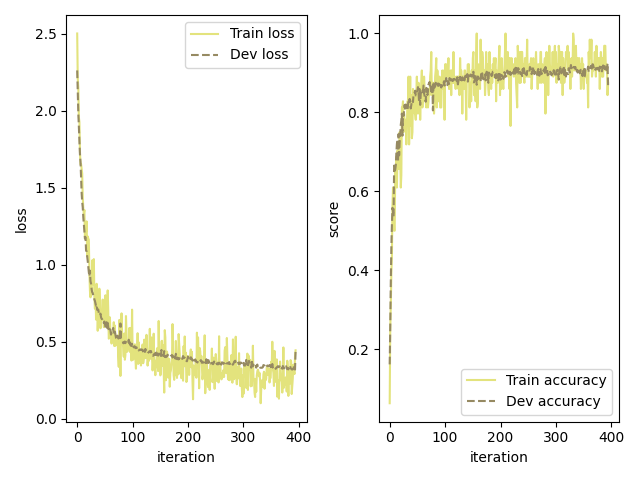
\includegraphics[width=0.72\linewidth]{figures/mlp_sgd_curve.png}
\caption{Part A learning curve for the MLP baseline.}
\label{fig:mlp-curve}
\end{figure}

The MLP learns a reasonable baseline for MNIST, reaching 89.70\% validation accuracy and 89.98\% test accuracy. The learning curve shows a clear decrease in training and validation loss during the early iterations, followed by a slower improvement phase. The training accuracy is slightly higher than the validation accuracy, which is expected because the model is optimized directly on the training subset. The gap is not very large, so the baseline does not appear to be severely overfitting under this short training setting.

The main limitation of this MLP is its input representation. Each image is flattened into a 784-dimensional vector, so neighboring pixels in the original image are not explicitly represented as neighbors in the model. The MLP can still learn useful digit patterns, but it has to learn spatial relationships through dense weights. This makes it a good baseline, but not the most natural model for image data.

\section{Part B: CNN Model}

\subsection{Required Implementation}

The CNN uses one convolutional layer followed by ReLU, flattening, and a final linear classifier:
\[
1 \times 28 \times 28 \xrightarrow{\mathrm{Conv}(8,5,1,2)} 8 \times 28 \times 28
\xrightarrow{\mathrm{ReLU}} \mathrm{Flatten} \rightarrow 10.
\]

The implemented \texttt{conv2D} operator supports input tensors of shape $[N,C,H,W]$, square kernels, stride, and zero padding. Its forward pass extracts local image patches with an \texttt{im2col}-style view and multiplies them by reshaped convolution kernels. The backward pass computes gradients for the kernels, biases, and input image tensor, then scatters patch gradients back to the padded image. This keeps the operator self-implemented while remaining efficient enough for the experiment.

The convolution layer is designed to preserve the two-dimensional structure of the image. A kernel is applied to local patches of the input, and the same kernel weights are reused at different spatial locations. This weight sharing is the key difference from the MLP: instead of learning unrelated weights for every input pixel position, the CNN learns local detectors that can respond to similar patterns anywhere in the image. In MNIST, such local patterns often correspond to short strokes, corners, loops, and edges.

The CNN used here is intentionally small. It has only one convolutional layer and one classifier layer, so the comparison focuses on the effect of adding convolution rather than on building a very deep or highly tuned network. He initialization is used for both MLP and CNN layers to keep activations at a more stable scale when using ReLU.

\subsection{MLP-vs-CNN Comparison}

\begin{table}[H]
\centering
\caption{Part B comparison under the same dataset split, batch size, and number of epochs.}
\label{tab:cnn-comparison}
\begin{tabular}{lccccc}
\toprule
Model & Optimizer & Train acc. & Validation acc. & Test acc. & Test loss \\
\midrule
MLP baseline & SGD & 0.9094 & 0.8970 & 0.8998 & 0.3415 \\
CNN baseline & SGD & 0.9216 & 0.9160 & 0.9075 & 0.3130 \\
\bottomrule
\end{tabular}
\end{table}

\begin{figure}[H]
\centering
\begin{subfigure}{0.48\textwidth}
\centering
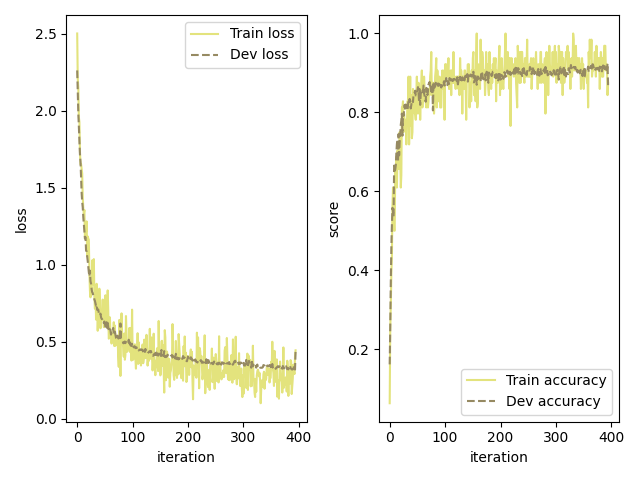
\includegraphics[width=\linewidth]{figures/mlp_sgd_curve.png}
\caption{MLP baseline}
\end{subfigure}
\begin{subfigure}{0.48\textwidth}
\centering
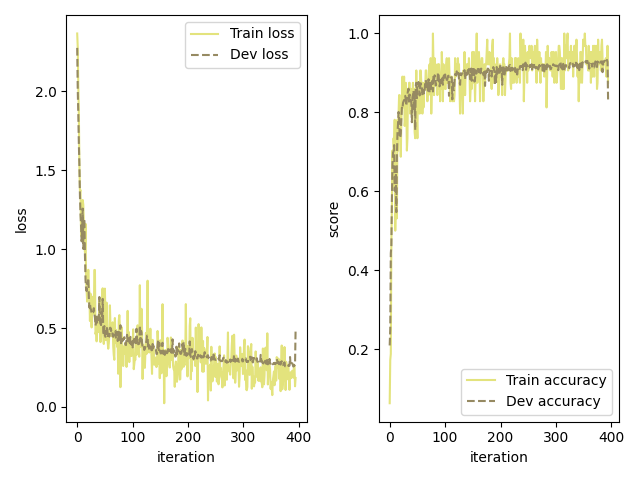
\includegraphics[width=\linewidth]{figures/cnn_sgd_curve.png}
\caption{CNN baseline}
\end{subfigure}
\caption{Part B learning curves for the MLP and CNN baselines.}
\label{fig:partb-curves}
\end{figure}

The CNN baseline outperforms the MLP baseline on validation accuracy and test accuracy. The validation accuracy increases from 89.70\% to 91.60\%, and the test accuracy increases from 89.98\% to 90.75\%. The improvement is moderate because the CNN is intentionally simple, but it is consistent with the image structure of MNIST.

The comparison suggests that even a shallow CNN benefits from an image-specific inductive bias. A CNN learns local filters that are shared across spatial positions, so the same stroke or corner detector can be useful in many parts of an image. The MLP must learn such spatial relationships from flattened pixels, which is less parameter-efficient. The CNN also achieves a lower test loss than the MLP, indicating that its predictions are not only more accurate but also better calibrated under the cross-entropy objective.

\section{Part C: Two Additional Directions}

I choose Direction 1, optimization, and Direction 2, regularization. These two directions are useful because they study different aspects of model performance. Optimization changes how the model searches for good parameters, while regularization changes the training objective to discourage overly large weights. To make Part C clearly build on both required parts, I apply the two directions to the MLP from Part A and the CNN from Part B. This gives a stricter comparison than only improving the best model: it shows whether the same idea behaves similarly across two different architectures.

\subsection{Direction 1: Optimization with Momentum}

For the optimization direction, I implement momentum gradient descent:
\[
v_t = \mu v_{t-1} - \eta \nabla_\theta L,\quad
\theta_t = \theta_{t-1}+v_t.
\]
The comparison baselines are the original MLP and CNN trained with plain SGD and weight decay. Momentum uses $\mu=0.9$ and learning rate 0.03. The architecture, dataset split, batch size, and number of epochs are kept fixed within each model family.

\begin{table}[H]
\centering
\caption{Part C Direction 1: optimization comparison.}
\label{tab:momentum}
\begin{tabular}{lccccc}
\toprule
Model & Optimizer & Train acc. & Validation acc. & Test acc. & Test loss \\
\midrule
MLP baseline & SGD & 0.9094 & 0.8970 & 0.8998 & 0.3415 \\
MLP + Momentum & Momentum & 0.9750 & 0.9390 & 0.9349 & 0.2173 \\
CNN baseline & SGD & 0.9216 & 0.9160 & 0.9075 & 0.3130 \\
CNN + Momentum & Momentum & 0.9962 & 0.9610 & 0.9644 & 0.1228 \\
\bottomrule
\end{tabular}
\end{table}

Momentum gives the clearest improvement in this project. For the MLP, test accuracy improves from 89.98\% to 93.49\%. For the CNN, test accuracy improves from 90.75\% to 96.44\%. The training accuracy also becomes much higher for both models, which means the optimizer finds a better solution within the same five-epoch budget. The learning curves in Figure~\ref{fig:partc-curves} show faster convergence and lower final losses.

This result is reasonable because mini-batch gradients are noisy. Plain SGD updates parameters using only the current gradient, so its direction can fluctuate from batch to batch. Momentum accumulates a velocity vector, which preserves directions that are repeatedly supported by recent gradients and reduces the influence of isolated noisy updates. In this experiment, both the MLP and CNN benefit from this effect, and the CNN benefits the most.

\subsection{Direction 2: Regularization with L2 Weight Decay}

For the regularization direction, I compare each relevant setting with and without L2 weight decay. For the MLP and CNN baselines, the comparison is SGD with $\lambda=10^{-4}$ versus SGD with $\lambda=0$. I also include the CNN+Momentum comparison because it is the strongest model in the report. The implemented weight decay multiplies each optimizable parameter by $(1-\eta\lambda)$ before applying the gradient update.

\begin{table}[H]
\centering
\caption{Part C Direction 2: L2 regularization comparison.}
\label{tab:regularization}
\begin{tabular}{lccccc}
\toprule
Setting & Weight decay & Train acc. & Validation acc. & Test acc. & Test loss \\
\midrule
MLP + SGD & $10^{-4}$ & 0.9094 & 0.8970 & 0.8998 & 0.3415 \\
MLP + SGD & 0 & 0.9094 & 0.8970 & 0.8996 & 0.3412 \\
CNN + SGD & $10^{-4}$ & 0.9216 & 0.9160 & 0.9075 & 0.3130 \\
CNN + SGD & 0 & 0.9216 & 0.9160 & 0.9075 & 0.3128 \\
CNN + Momentum & $10^{-4}$ & 0.9962 & 0.9610 & 0.9644 & 0.1228 \\
CNN + Momentum & 0 & 0.9962 & 0.9620 & 0.9647 & 0.1226 \\
\bottomrule
\end{tabular}
\end{table}

In this short subset experiment, L2 weight decay does not produce a meaningful improvement for either architecture. For the MLP baseline, the test accuracy changes from 89.98\% to 89.96\% after removing weight decay. For the CNN baseline, the test accuracy remains 90.75\%. For the CNN+Momentum model, the no-weight-decay run is higher by only 0.03 percentage points on the test set, which is too small to treat as a reliable advantage. The train accuracy, validation accuracy, and loss values are also nearly identical in each pair.

There are several possible explanations. First, the model is small and trained for only five epochs, so the regularization effect may not have enough time to become visible. Second, the selected value $\lambda=10^{-4}$ may be too weak to noticeably change the learned parameters. Third, MNIST is relatively simple, so this model may generalize well even without explicit weight decay. Therefore, the correct conclusion is not that weight decay is useless in general, but that this particular setting does not show a measurable benefit from it.

\begin{figure}[H]
\centering
\begin{subfigure}{0.48\textwidth}
\centering
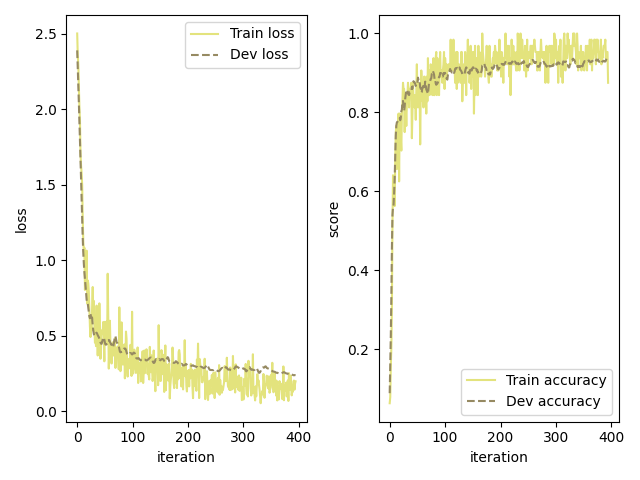
\includegraphics[width=\linewidth]{figures/mlp_momentum_curve.png}
\caption{MLP with momentum}
\end{subfigure}
\begin{subfigure}{0.48\textwidth}
\centering
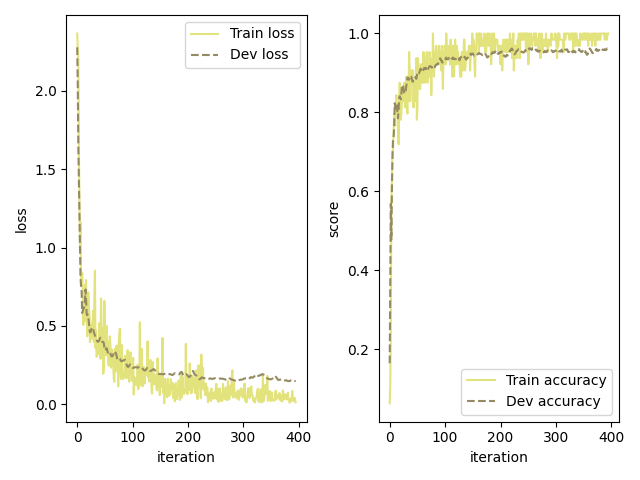
\includegraphics[width=\linewidth]{figures/cnn_momentum_curve.png}
\caption{CNN with momentum}
\end{subfigure}
\begin{subfigure}{0.48\textwidth}
\centering
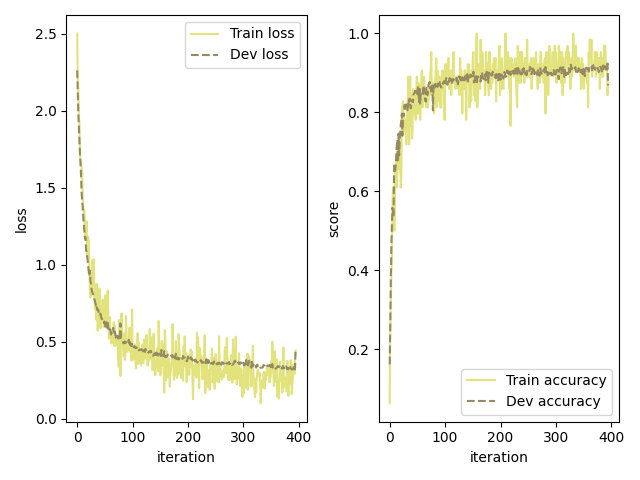
\includegraphics[width=\linewidth]{figures/mlp_no_wd_curve.png}
\caption{MLP without weight decay}
\end{subfigure}
\begin{subfigure}{0.48\textwidth}
\centering
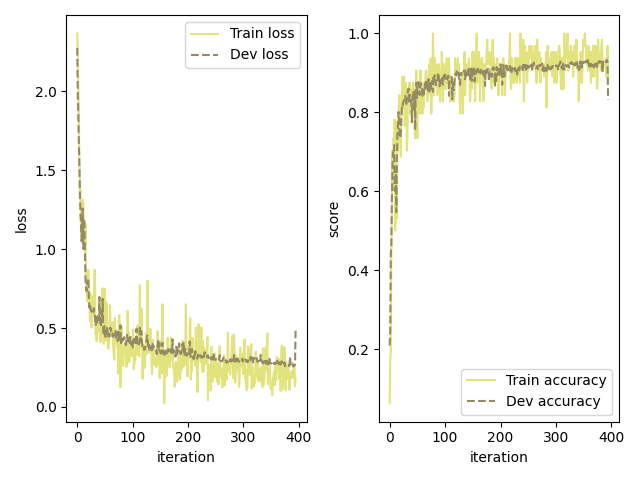
\includegraphics[width=\linewidth]{figures/cnn_sgd_no_wd_curve.png}
\caption{CNN without weight decay}
\end{subfigure}
\caption{Part C learning curves for optimization and regularization studies on both MLP and CNN.}
\label{fig:partc-curves}
\end{figure}

\section{Main Results Table}

\begin{table}[H]
\centering
\caption{Summary of all required and additional experiments.}
\label{tab:main-results}
\small
\begin{tabular}{llllccc}
\toprule
Part & Experiment & Model & Optimizer & Weight decay & Val acc. & Test acc. \\
\midrule
A & MLP baseline & MLP & SGD & $10^{-4}$ & 0.8970 & 0.8998 \\
B & CNN baseline & CNN & SGD & $10^{-4}$ & 0.9160 & 0.9075 \\
C1 & Optimization & MLP & Momentum & $10^{-4}$ & 0.9390 & 0.9349 \\
C1 & Optimization & CNN & Momentum & $10^{-4}$ & 0.9610 & 0.9644 \\
C2 & Regularization control & MLP & SGD & 0 & 0.8970 & 0.8996 \\
C2 & Regularization control & CNN & SGD & 0 & 0.9160 & 0.9075 \\
C2 & Regularization control & CNN & Momentum & 0 & 0.9620 & 0.9647 \\
\bottomrule
\end{tabular}
\end{table}

\section{Requirement Checklist}

\begin{table}[H]
\centering
\caption{Project requirement checklist.}
\label{tab:checklist}
\footnotesize
\begin{tabular}{p{0.25\linewidth}p{0.58\linewidth}p{0.08\linewidth}}
\toprule
Requirement & How it is satisfied & Status \\
\midrule
Part A: implement linear forward/backward & Implemented in the Linear layer. & Done \\
Part A: implement softmax cross-entropy & Implemented in the multi-class cross-entropy loss layer. & Done \\
Part A: train MLP and report train/validation performance & MLP results and learning curve are reported in Table~\ref{tab:mlp} and Figure~\ref{fig:mlp-curve}. & Done \\
Part B: implement \texttt{conv2D} & Implemented self-contained NumPy convolution forward/backward. & Done \\
Part B: build CNN and compare with MLP & CNN results are compared against MLP in Table~\ref{tab:cnn-comparison}. & Done \\
Part C: choose two directions & Chosen directions are optimization and regularization. & Done \\
Part C: compare with appropriate baselines & Momentum and weight decay are tested on both MLP and CNN settings. & Done \\
Main results table & All required and additional results are summarized in Table~\ref{tab:main-results}. & Done \\
Detailed visualization & Learning curves, confusion matrix, convolution kernels, and misclassified examples are included. & Done \\
\bottomrule
\end{tabular}
\end{table}

\section{Detailed Visualization}

\begin{figure}[H]
\centering
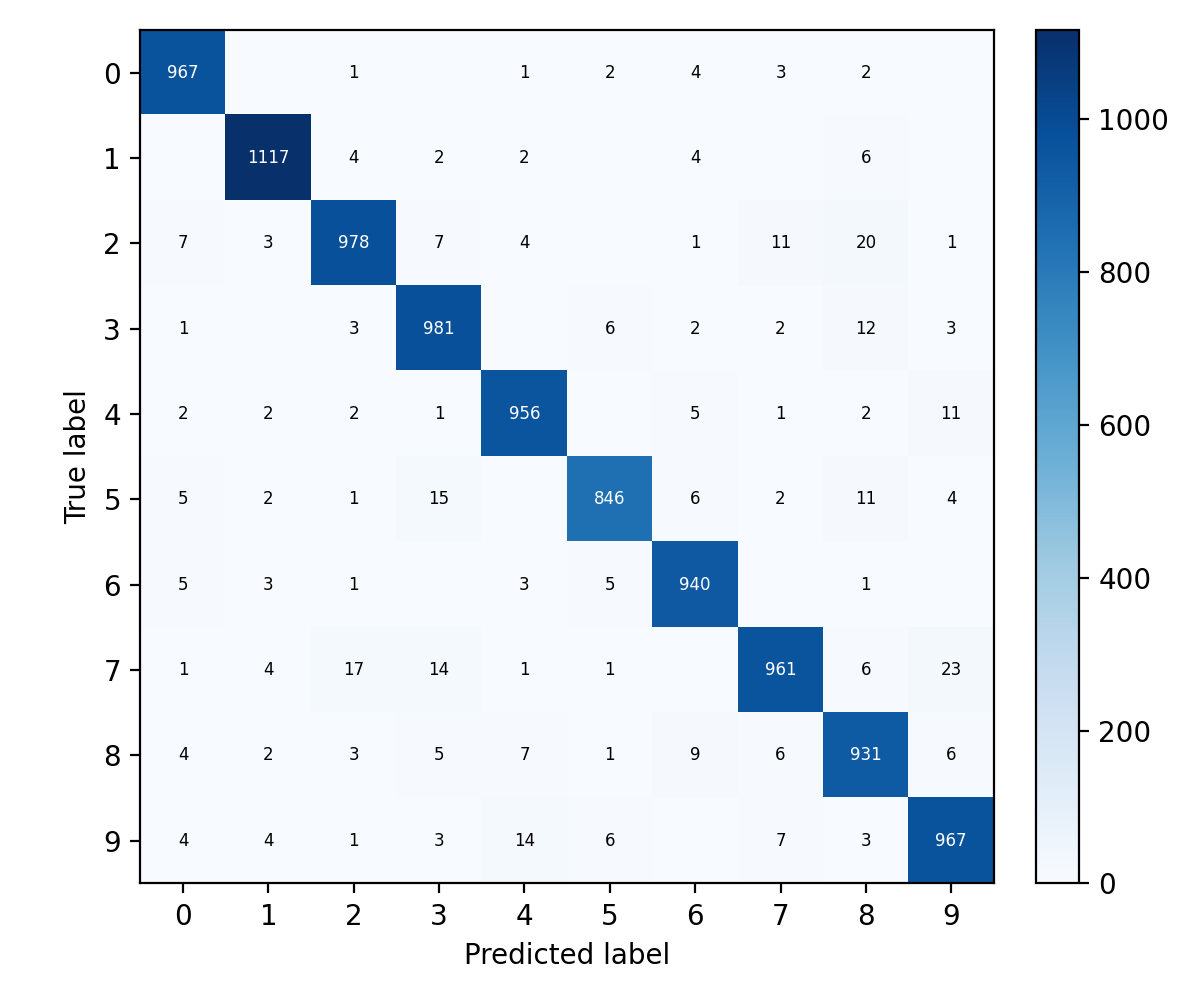
\includegraphics[width=0.72\linewidth]{figures/confusion_matrix.png}
\caption{Confusion matrix of the CNN+Momentum model on the full MNIST test set.}
\label{fig:confusion}
\end{figure}

The confusion matrix is dominated by the diagonal, showing that the CNN+Momentum model classifies most test images correctly. The remaining off-diagonal entries reveal the most common confusion patterns. For example, some 2s are predicted as 8 or 9, and some 7s are predicted as 2, 3, or 9. These mistakes usually occur when the written digit has an unusual stroke shape or when a digit lacks a clear distinguishing component.

\begin{figure}[H]
\centering
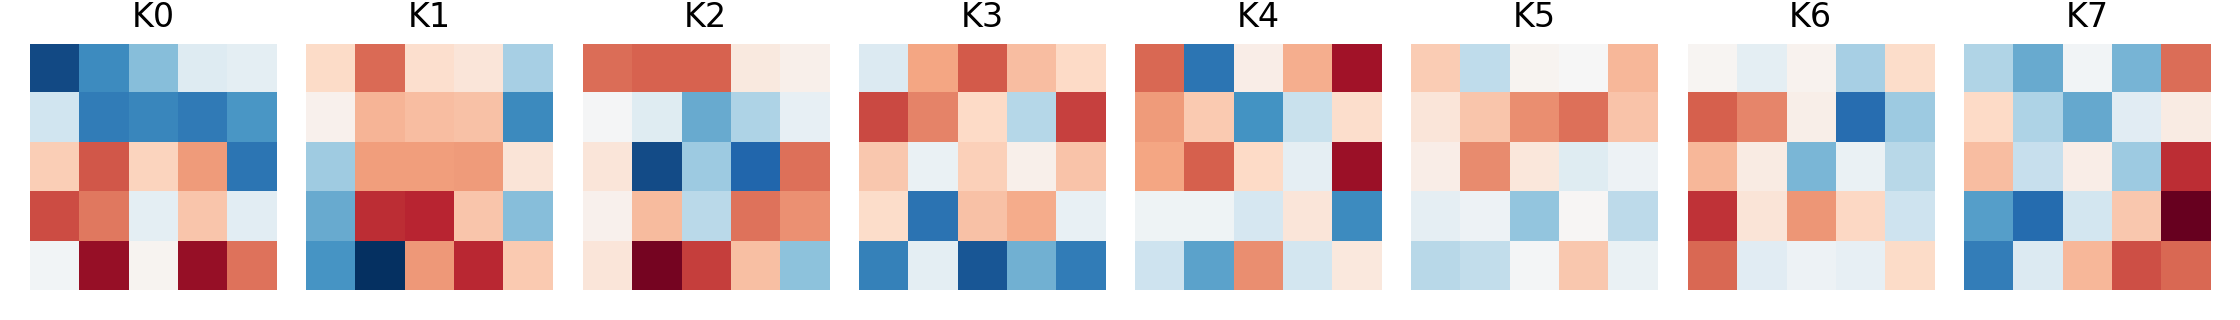
\includegraphics[width=0.9\linewidth]{figures/conv_kernels.png}
\caption{Learned convolution kernels in the CNN+Momentum model. The filters capture simple local stroke and edge-like patterns.}
\label{fig:kernels}
\end{figure}

The learned convolution kernels show that the model has learned small local templates. Although the filters are not directly human-readable as complete digits, they contain positive and negative regions that respond to local contrast patterns. This is consistent with the role of the first convolutional layer: it should detect low-level stroke fragments rather than whole digit classes.

\begin{figure}[H]
\centering
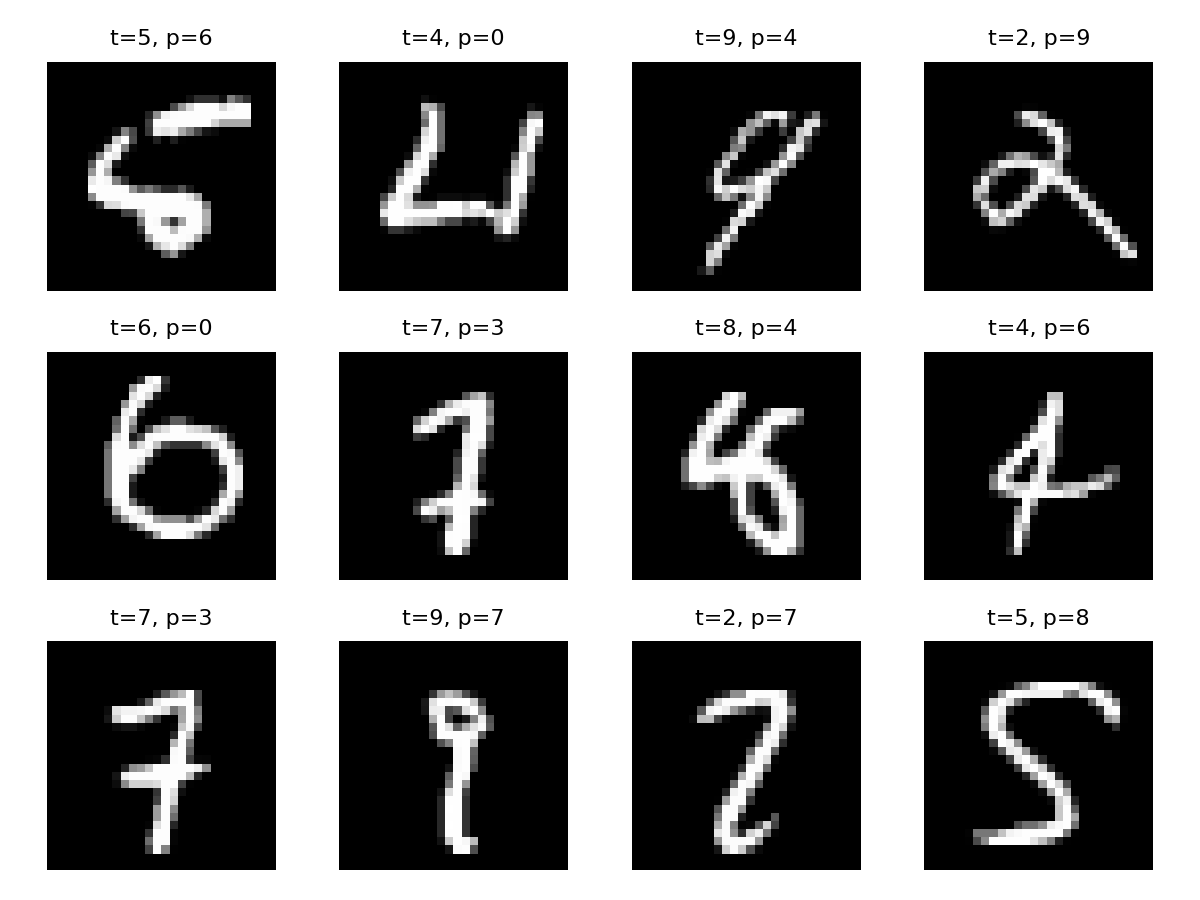
\includegraphics[width=0.85\linewidth]{figures/misclassified_examples.png}
\caption{Examples misclassified by the CNN+Momentum model. Many errors are visually ambiguous or have unusual handwriting styles.}
\label{fig:misclassified}
\end{figure}

The misclassified examples support the same conclusion. Many of the errors are visually ambiguous even for a human observer. Some samples are written with broken strokes, unusual curves, or shapes that resemble another digit. This suggests that the remaining errors are not only due to the model architecture, but also due to intrinsic ambiguity in some handwritten samples.

\section{Discussion}

The required MLP baseline, CNN model, and two additional directions are all completed. The experiments answer the main questions of the project. First, the MLP is a valid baseline and can classify MNIST reasonably well, but it treats each image as a flat vector. Second, the CNN is more suitable for image classification because it preserves local spatial structure and shares filters across positions. This gives better validation and test accuracy under the same data split and number of epochs.

Among the two additional directions, optimization is more informative in this experiment. Momentum significantly improves convergence and final accuracy for both the MLP and the CNN. This means the optimization conclusion is not limited to one architecture. The L2 regularization comparison is less decisive: both with and without weight decay produce almost identical train, validation, and test accuracy for the MLP baseline, CNN baseline, and CNN+Momentum model. This indicates that the chosen models and training duration are not strongly limited by overfitting in this setting.

The hard samples are mostly ambiguous handwritten digits. The confusion matrix and misclassified examples show errors such as 5/6, 7/3, 2/7, and 9/4, where the digit shape can be visually close to another class. Training on the full 60000 images, using a deeper CNN, or adding data augmentation would likely improve robustness.

One limitation of this report is that the experiments use a subset of the training set rather than all 60000 training images. This makes the NumPy experiments manageable, especially for the self-implemented convolution operator, but the reported accuracy should be interpreted as a controlled comparison rather than the best possible MNIST result. Another limitation is that each setting is run once with a fixed random seed. Repeating the experiments with multiple seeds would make the conclusions about small differences, especially weight decay, more reliable.

\section{Conclusion}

This submission completes Part A, Part B, and two Part C directions. The implemented NumPy MLP reaches 89.98\% test accuracy, and the self-implemented CNN baseline reaches 90.75\%. For Part C, momentum optimization improves the MLP to 93.49\% and the CNN to 96.44\%, showing a clear optimization benefit on both models. L2 weight decay is implemented and evaluated on both MLP and CNN settings, but it does not show a meaningful benefit in this particular short experiment.

\end{document}
